\documentclass[12pt,a4paper]{article}
\usepackage[margin=0.92in]{geometry}
\usepackage[T1]{fontenc}
\usepackage[utf8]{inputenc}
\usepackage{lmodern}
\usepackage{amsmath,amssymb,booktabs,array,graphicx,hyperref,xcolor,enumitem,microtype}
\usepackage[backend=biber,style=numeric,sorting=none]{biblatex}
\addbibresource{references.bib}
\usepackage{pgfplots}
\pgfplotsset{compat=1.18}
\hypersetup{colorlinks=true,urlcolor=blue!60!black,linkcolor=blue!60!black,citecolor=blue!60!black}
\setlength{\parskip}{4pt}
\setlength{\parindent}{0pt}
\emergencystretch=2em
\setlist[itemize]{noitemsep,topsep=3pt,leftmargin=1.35em}
\setlist[enumerate]{noitemsep,topsep=3pt,leftmargin=1.6em}
\newcommand{\pre}{\textsc{Pre}}
\newcommand{\post}{\textsc{Post}}
\newcommand{\NA}{\textsc{NA}}
\title{Evaluating Claim-Level Temporal and Citation Verification in Retrieval-Augmented Scientific Synthesis\\[5pt]\large An Exploratory Fixed-Context Study and a Local-Model Challenge Extension}
\author{Lodha Krunal Rajubhai\\\small M.Tech -- AI Tools for Research, IIIT Allahabad}
\date{November 2026}
\begin{document}
\maketitle
\begin{abstract}
Scientific literature reviews generated by language models can appear well grounded even when their cited evidence is either unsupported or too recent for a historical question. We examine a narrower issue: can a claim-level verifier remove citations that violate a fixed knowledge cutoff without discarding admissible claims? Our first experiment used 11 fixed-context questions, each paired with four source passages dated before 30 June 2025 and four dated afterward. Across the saved baseline responses, we recorded 85 claims and 86 citation links; every citation pointed to a pre-cutoff source version. A single, nonblind AI review provisionally judged all 85 claims supported, but this was not independent annotation. The four archived verifier responses retained all 31 claims they assessed. The remaining seven cases relied on author confirmations or same-conversation assessments, so the full ledger of 85 retained claims cannot be treated as 11 independent verifier runs. With no post-cutoff citation observed in the baseline, the verifier had no date error to correct. We therefore report this result as a floor effect, not as evidence that verification is unnecessary. In a separate exploratory extension, we ran Qwen2.5 3B on seven reused questions with stricter and weaker cutoff prompts. Post-cutoff versions were cited in 16 of 51 strict-prompt claims and 20 of 39 weak-prompt claims. A deterministic date rule removed all 20 such weak-prompt claims by construction. The Qwen verifier removed 7 of 20 but incorrectly rejected two pre-only claims as post-cutoff; on strict-prompt claims it removed 4 of 16 post-cutoff-citing claims and incorrectly rejected 18 pre-only claims for the same reason. These findings concern source-version dates, not independently confirmed factual support or gold-fact coverage. The accompanying code, saved records and provenance notes allow these limitations and results to be checked.
\end{abstract}

\noindent\textbf{Keywords:} historical knowledge cutoff, literature synthesis, scientific question answering, retrieval-augmented generation, citation support, claim verification, temporal leakage.

\section{Introduction}
Language models can produce readable literature reviews in a short time. The harder question is whether their claims are supported by the right evidence. A reference may be bibliographically valid---that is, it identifies a real publication---yet still fail to support the sentence attached to it. Earlier evaluations have examined reference matching against bibliographic databases and academic search \cite{tang2025}, while OpenScholar assessed whether citations to individual statements were appropriate and supportive \cite{asai2024}. For a question set at a historical date, there is another requirement: even a genuine, relevant source may be inadmissible if the supplied version appeared after that date.

Retrieval can bring relevant publications into a model's context, as illustrated by LitLLM's search-and-rerank workflow \cite{agarwal2025} and OpenScholar's retrieval, feedback and citation-checking process \cite{asai2024}. Other work evaluates the structure of generated review tables \cite{newman2024} or the coherence and reference overlap of generated surveys \cite{shi2025}. These are useful quality measures, but none can replace a direct check that the particular evidence cited for a historical claim existed by the chosen cutoff.

\textbf{Research question.} Given the same pre- and post-cutoff passages, can a verifier applied after generation remove inadmissible or unsupported claims while preserving claims backed by eligible historical evidence? We first compare a cutoff-constrained generator (Baseline A) with a deletion-only verifier (B) acting on A's saved claims. The passages are curated and fixed in advance; this is a controlled stress test, not a test of retrieval quality or a reproduction of a complete published system.

\textbf{What we observed.} In Experiment~1 the constrained baseline cited only pre-cutoff versions, leaving the verifier with no observed date violations to remove. The saved B decisions also have mixed provenance, so they cannot establish a benefit from verification. To learn more about behavior when mistakes do occur, we conducted a separate local-model extension with strict and weak prompting and two filtering methods. Because the models and procedures differ, we analyze the experiments separately rather than pooling their results.

\section{Related Work and Verified Motivation}
\textbf{Retrieval-grounded scientific synthesis.} LitLLM addressed hallucinations and missing recent work through query expansion, web retrieval and reranking \cite{agarwal2025}. OpenScholar combined scientific retrieval with iterative feedback and citation verification and introduced SCHOLARQABENCH for evaluating scientific synthesis \cite{asai2024}. These systems provide useful reference points for our study because they treat evidence selection and citation quality as part of the generation process rather than relying on fluent text alone.

\textbf{What the metrics measure.} Tang et al. assessed generated references through database matching, precision, recall, F1 and external title search, while separately evaluating the consistency and coverage of review text \cite{tang2025}. OpenScholar instead evaluated whether citations attached to statements were necessary and supportive \cite{asai2024}. Studies of ROUGE and key-point recall show why lexical similarity alone cannot stand in for evidence coverage \cite{ali2024,tang2025}. We therefore record citation dates and claim support separately: a correct publication date does not prove that a citation supports its claim.

\textbf{Other review-generation settings.} ARXIVDIGESTABLES generated structured literature tables from titles and abstracts and measured schema alignment, while acknowledging limitations associated with arXiv-only and English-language inputs \cite{newman2024}. SciSage explored multiagent survey drafting and revision, using reference overlap and human judgments of coherence among its evaluations \cite{shi2025}. We draw on these different tasks to avoid limiting the historical questions to one style of review generation.

\section{Research Design}
\subsection{Historical cutoff and evidence corpus}
The historical cutoff is \textbf{30 June 2025 at 23:59:59 UTC}. We worked with \textbf{11 version-specific PDFs}: six versions available by the cutoff and five dated later. Eligibility follows the date of the \emph{exact document version} provided, not the date of an earlier version or the paper's general publication year. All 11 original PDF SHA-256 hashes matched the existing source manifest. The six eligible versions correspond to papers cited in our references \cite{agarwal2025,newman2024,asai2024,ali2024,tang2025,shi2025}; later versions were deliberately included as distractors but could not serve as historical support.

The original design contains 13 curated contexts: two development cases and 11 held-out questions (H01--H07 and H09--H12). We excluded D03 and H08 after noticing overlap concerns. Each question has eight passages in a fixed order, with four from eligible versions and four from later versions. We deliberately included two pre-cutoff anchor passages per question, but that design choice should not be mistaken for measured retrieval recall or independently verified gold-fact coverage. Extracted passages underwent visual review and limited cleanup before held-out generation. In two cases, we manually replaced the initially selected TF--IDF passage for quality reasons and recorded those departures from automatic selection.

Not every original interface submission could be reconstructed byte for byte. Some passage contexts were recovered from saved prompt files and an earlier checked repair candidate. We checked A's cited IDs against each question's source registry and compared relevant cited spans with the supplied passages and original PDFs. For four restored contexts, however, the repaired material cannot be certified as identical to the prompt actually pasted into the interface. This remains a reproducibility limitation.

\subsection{Compared arms and invariant}
\textbf{Baseline A} receives the question and all eight passages, with explicit instructions to avoid external sources and cite only exact pre-cutoff source IDs. It may return no claims or up to eight original factual claim records in JSON, each with a consecutive ID, text and citation list. The saved answer is the immutable input to Verifier B.

\textbf{Verifier B} sees the identical question and evidence together with A's \emph{exact recorded claims}. B can label each claim \texttt{KEEP}, \texttt{DROP\_POST\_CUTOFF}, \texttt{DROP\_UNSUPPORTED} or \texttt{DROP\_UNCERTAIN}; it may not rewrite, add or reorder claims. The software guard checks that its retained IDs form the same-order subset of A IDs. This design isolates post-generation deletion, although it cannot increase coverage by adding missing pre-cutoff facts. The reported ChatGPT interface model selection was GPT-6 Thinking; the exact model build, temperature and seed were not visible. Tool browsing was prohibited by prompt, but interface execution details were not fully logged.

\subsection{Saved run provenance}
The saved B records do not all have the same provenance. For H01, H02, H03 and H12, we have separately pasted verifier JSON responses. For H06 and H07, the author confirmed that all seven claims were kept, but separate original response files were not preserved. H04, H05, H09, H10 and H11 were assessed in a conversation where the assistant had already seen A's outputs. We therefore treat the four archived responses as the clearest paired evidence and use the 11-case ledger only for descriptive accounting. The other seven entries do \emph{not} satisfy the planned fresh-chat independence requirement.

\subsection{Claim annotation and metrics}
Our scoring unit is the original saved claim \emph{record}, rather than post hoc split atomic subclaims. Source-support labels are \texttt{SUPPORTED}, \texttt{UNSUPPORTED} and \texttt{UNCERTAIN}; cited-source temporal labels include \texttt{PRE\_ONLY}, \texttt{POST\_ONLY} and \texttt{MIXED}. A source-date pass checks citation admissibility structurally, while claim-support annotation asks whether the cited text actually entails the claim. These checks must not be conflated.

The primary, lower-is-better metric for an arm $X$ is
\begin{equation}
 R_{\mathrm{post}}(X)=\frac{\#\{\text{supported claim records dependent only on post-cutoff cited evidence}\}}{\#\{\text{supported claim records in }X\}}.
\label{eq:main}
\end{equation}
If the denominator is zero, $R_{\mathrm{post}}$ is \NA, never automatically zero. Auxiliary measures include retained and deleted claim counts, unsupported and uncertain counts, and an overfiltering rate defined as valid pre-only supported A records deleted by B divided by all valid pre-only supported A records. Strict citation-pair precision and gold-fact coverage require separate annotations; we leave them \NA\ rather than equating 86 syntactically valid citation links with 86 independent gold matches.

One assistant reviewed all 85 saved claims against their cited passages after the A and B outputs were available. These are useful preliminary support judgments, but the reviewer was not blind and no independent human annotated the same material. We therefore do not present them as gold accuracy. The scoring script summarizes saved outputs and provisional labels; it does not generate or recover missing responses.

\section{Results}
\subsection{Structural integrity and pre-cutoff citation compliance}
Across the 11 saved A responses, we counted \textbf{85 claim records} and \textbf{86 citation links}. Each cited ID appears in its question's evidence registry and identifies a source version dated before 1 July 2025. We therefore found no post-cutoff citations in these outputs. The later, nonblind assistant review marked 85/85 records as supported, with none marked unsupported or uncertain. This is a \emph{provisional} assessment, not independently established ground truth.

\begin{table}[ht]
\centering\small
\caption{Reported A/B records. B provenance is central to interpreting the totals.}
\label{tab:cases}
\begin{tabular}{lrrrrl}
\toprule
Case & A & B kept & B drop & Post-only A & B source\\
\midrule
H01 & 7 & 7 & 0 & 0 & Original user-pasted\\
H02 & 8 & 8 & 0 & 0 & Original user-pasted\\
H03 & 8 & 8 & 0 & 0 & Original user-pasted\\
H04 & 8 & 8 & 0 & 0 & Assistant in-chat\\
H05 & 8 & 8 & 0 & 0 & Assistant in-chat\\
H06 & 7 & 7 & 0 & 0 & Author-confirmed\\
H07 & 7 & 7 & 0 & 0 & Author-confirmed\\
H09 & 8 & 8 & 0 & 0 & Assistant in-chat\\
H10 & 8 & 8 & 0 & 0 & Assistant in-chat\\
H11 & 8 & 8 & 0 & 0 & Assistant in-chat\\
H12 & 8 & 8 & 0 & 0 & Original user-pasted\\
\midrule
\textbf{All, mixed provenance} & \textbf{85} & \textbf{85} & \textbf{0} & \textbf{0} & Not 11 independent runs\\
\bottomrule
\end{tabular}
\end{table}

\subsection{Paired outcomes and a floor effect}
The four cases with preserved B response JSONs contain 31 claims, all of which were kept. Author confirmations account for another 14 KEEP decisions, and same-conversation assessments account for 40. The complete ledger consequently records \textbf{85/85 claims retained}, but this combined number describes records of unequal provenance. It does not turn the seven less independently documented cases into preserved verifier runs.

Using the provisional support labels, both arms have $R_{\mathrm{post}}=0/85=0$ in the mixed-provenance ledger. Their absolute difference is \textbf{zero percentage points}; a relative reduction cannot be calculated when the baseline error rate is already zero. Because no records were deleted, provisional overfiltering is also 0/85. Gold-fact coverage and strict citation-pair precision are not reported as validated metrics; latency and monetary cost were not measured.

\begin{figure}[ht]
\centering
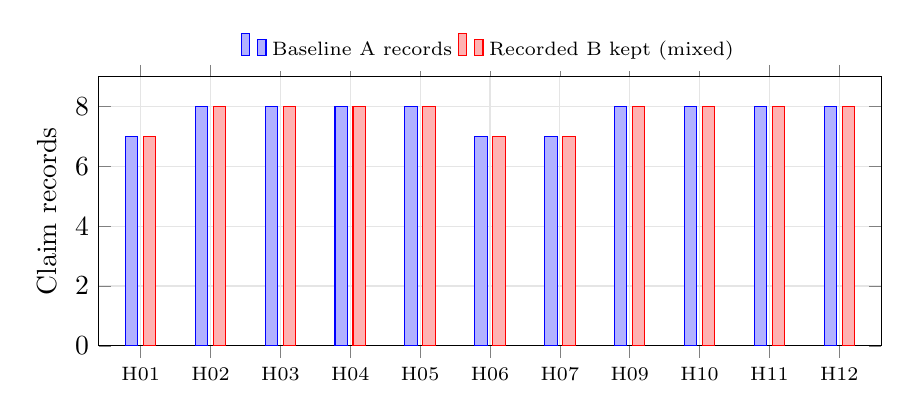
\begin{tikzpicture}
\begin{axis}[
 width=0.95\linewidth,height=5.0cm,ymin=0,ymax=9,
 symbolic x coords={H01,H02,H03,H04,H05,H06,H07,H09,H10,H11,H12},
 xtick=data,xticklabel style={font=\scriptsize},
 ytick={0,2,4,6,8}, ylabel={Claim records},
 ybar,bar width=4.5pt, enlarge x limits=0.06,
 legend style={at={(0.5,1.02)},anchor=south,legend columns=2,font=\scriptsize,draw=none},
 grid=major,grid style={gray!20}]
\addplot coordinates {(H01,7)(H02,8)(H03,8)(H04,8)(H05,8)(H06,7)(H07,7)(H09,8)(H10,8)(H11,8)(H12,8)};
\addplot coordinates {(H01,7)(H02,8)(H03,8)(H04,8)(H05,8)(H06,7)(H07,7)(H09,8)(H10,8)(H11,8)(H12,8)};
\legend{Baseline A records,Recorded B kept (mixed)}
\end{axis}
\end{tikzpicture}
\caption{Saved original claim counts and recorded B retention counts are identical in all 11 cases. The B bar is a mixture of raw outputs, author confirmations and same-conversation assessments; the plot is descriptive, not a claim of 11 independent verifier runs.}
\label{fig:retention}
\end{figure}

\subsection{Traceable examples from genuine pasted B-response cases}
Table~\ref{tab:examples} illustrates why the retained-claim ledger cannot be treated as a hidden performance gain. Every example is taken from one of the four questions with individually pasted B output rather than the assistant-only assessment group. The cited sources predate the cutoff and substantiate the specific claim; B's decision is a retention, not an independently measured verification correction.

\begin{table}[ht]
\centering\small
\caption{Three original A claim records, their cited evidence and preserved B decisions.}
\label{tab:examples}
\begin{tabular}{p{0.11\linewidth}p{0.65\linewidth}p{0.10\linewidth}}
\toprule
Claim & Traceable claim and source & B \\
\midrule
H01 C05 & A generated bibliographic reference counted as reliable if its title and another metadata field matched, or if a wrong title was offset by three matching metadata fields (\texttt{2412.13612v4\_p4\_c3}). & KEEP \\
H03 C02 & GPT-3.5-TURBO-0125 had ROUGE-1 0.364, versus 0.268 for T5 and 0.257 for spaCy (\texttt{2411.18583v1\_p5\_c1}). & KEEP \\
H12 C04 & A cited source gave F1 as the harmonic mean of precision and recall (\texttt{2506.12689v1\_p10\_c3}). & KEEP \\
\bottomrule
\end{tabular}
\end{table}

All three are intelligible examples of \emph{correctly retained} historical evidence rather than corrected baseline hallucinations. Since the experiment did not yield an observed temporal citation violation, it has no genuine held-out \texttt{DROP\_POST\_CUTOFF} error case to analyze. This constraint is reported, not hidden behind synthetic examples.


\section{Experiment 2: Exploratory Local-Model Challenge}
\label{sec:e2}
\subsection{Versioned extension and comparators}
Because Experiment~1 contained no baseline citation-date violations, it could not tell us how the verifier behaves when such errors are present. As an exploratory follow-up, we reused seven archived question--evidence contexts (H01, H02, H03, H06, H07, H09, H12). They are \emph{not a new held-out set}. We kept each question and its eight source versions, but moved the four post-cutoff passages ahead of the four pre-cutoff passages for every arm. The cutoff itself remained 30 June 2025, 23:59:59 UTC.

For this extension we ran \texttt{atr-qwen3b}, a local Ollama model derived from Qwen2.5 3B, with temperature 0 and requested seed 42. We could not independently establish the exact backend build or guarantee deterministic execution. The final \texttt{E2v4} runner enforced JSON schemas after an earlier H02 attempt returned claims without citation fields; the earlier attempts remain in the archive. We generated answers independently under two instructions. \emph{Strict A} explicitly prohibited citations to later versions, whereas \emph{weak A0} did not include that prohibition. Each produced at most eight claims. We then passed the saved outputs to fresh deletion-only verifier calls and separately applied a deterministic rule to A0 that removes any claim citing a post-cutoff or unknown source ID. The resulting five analysis arms are strict A, strict A+B, weak A0, weak A0+date rule and weak A0+B. Unlike the LLM verifier, the rule checks dates only and makes no claim about factual support.

For the main analysis, we used the first seven completed E2v4 runs \emph{reported by the researcher}, as listed in \texttt{E2v4\_primary\_run\_manifest.csv}. This selection was not preregistered and was not based on chronological order. In fact, an earlier successful H02 run is also archived. It has the same question and evidence hashes and the same requested model, temperature and seed, but different outputs. We keep both runs and report the sensitivity of the conclusions to H02 selection below. All main-table values were recalculated from the seven declared JSON records, not from an indiscriminate pool of eight completed runs.

\subsection{Observed citation-date comparisons}
\begin{table}[ht]
\centering\small
\setlength{\tabcolsep}{4pt}
\caption{Experiment 2 selected seven-run citation-date results. ``Post'' means a claim cited at least one post-cutoff source version. Correct/false date drops compare model decisions with source-version DATE, not with independent factual support. Dashes denote no deletion decision.}
\label{tab:e2_arms}
\begin{tabular}{p{0.26\linewidth}rrrrrr}
\toprule
Arm & Claims & Post & Kept & Correct drop & False drop & Post kept\\
\midrule
Strict A & 51 & 16 & 51 & -- & -- & 16\\
Strict A + Qwen B & 51 & 16 & 29 & 4 & 18 & 12\\
Weak A0 & 39 & 20 & 39 & -- & -- & 20\\
Weak A0 + date rule & 39 & 20 & 19 & 20 & 0 & 0\\
Weak A0 + Qwen B & 39 & 20 & 30 & 7 & 2 & 13\\
\bottomrule
\end{tabular}
\end{table}

Strict A generated 51 claims: 35 cited only pre-cutoff versions, and 16 cited at least one later version (13 post-only and three mixed-date). Weak A0 generated 39 claims, of which 20 cited later evidence. The corresponding citation-date violation proportions were 16/51 (31.4\%) and 20/39 (51.3\%). This difference is observable in our saved records, but the two prompts produced different claim counts and we reused only seven questions; it should not be generalized as a causal performance estimate. Weak A0 also abstained on H07, leaving that question's claim-level rates undefined.

The rule-based filter removed all 20 weak-A0 claims that cited later versions and kept all 19 pre-only claims, exactly as its date-checking logic specifies. That outcome shows correct source-date filtering, not factual verification. Qwen B removed only 7 of the 20 weak-arm claims with later citations and kept the other 13. It also marked two pre-only claims as \texttt{DROP\_POST\_CUTOFF}. For strict A, Qwen removed 4 of 16 post-cutoff-citing claims, kept 12, and mistakenly assigned the post-cutoff code to 18 of the 35 pre-only claims. These are \emph{source-date misclassifications}; without independent support review, we cannot call them gold-standard overfiltering. The observed post-citation detection proportions were 35\% (7/20) for weak A0 and 25\% (4/16) for strict A.

\begin{figure}[ht]
\centering
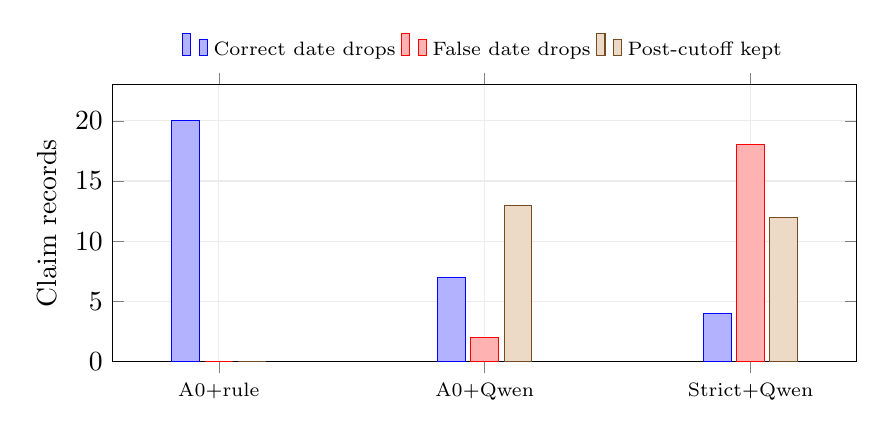
\begin{tikzpicture}
\begin{axis}[
 width=0.91\linewidth,height=5.1cm,ymin=0,ymax=23,
 xtick={1,2,3}, xticklabels={A0+rule,A0+Qwen,Strict+Qwen},
 xticklabel style={font=\scriptsize},
 ylabel={Claim records},ytick={0,5,10,15,20},
 ybar,bar width=10pt, enlarge x limits=0.20,
 legend style={at={(0.5,1.05)},anchor=south,legend columns=3,font=\scriptsize,draw=none},
 grid=major,grid style={gray!15}]
\addplot coordinates {(1,20)(2,7)(3,4)};
\addplot coordinates {(1,0)(2,2)(3,18)};
\addplot coordinates {(1,0)(2,13)(3,12)};
\legend{Correct date drops,False date drops,Post-cutoff kept}
\end{axis}
\end{tikzpicture}
\caption{Experiment 2 decision breakdown on the seven selected runs. Each ``correct'' or ``false'' label is verified only against recorded source-version dates; semantic citation support is not established.}
\label{fig:e2_decisions}
\end{figure}

\subsection{Sensitivity, failure cases and limits}
We also tested how much the results depend on which H02 completion is used. Substituting the earlier H02 run changes strict A from \textbf{16/51} to \textbf{20/53} post-cutoff-citing claims. For strict A+B, correct date drops increase from \textbf{4} to \textbf{5}, and the number of post-cutoff-citing claims still retained increases from \textbf{12} to \textbf{15}. Weak A0 remains at \textbf{20/39}, but weak A0+B changes from \textbf{7} to \textbf{6} correct drops and from \textbf{13} to \textbf{14} retained post-cutoff-citing claims. Incorrect date drops stay at 18 in the strict arm and two in the weak arm. The differences matter; because the selection rule was not preregistered, neither H02 run should be presented as an unquestionably privileged primary observation.

H01 illustrates the failure particularly clearly. Every strict-A claim cited \path{2411.14199v1_p10_c2}, which predates the cutoff, yet Qwen labelled all eight claims \texttt{DROP\_POST\_CUTOFF}. We can establish that the date reason was wrong; we cannot infer from dates alone that those eight claim texts were supported. H02 and H03 show a different problem: later sources were cited even under strict instructions. Because the passages were curated, only one local model and requested seed were tested, and claim-support adjudication was not part of this experiment, Experiment~2 supports \emph{source-date analysis only}. Supported-claim $R_{\mathrm{post}}$, strict factual citation precision and gold-validated overfiltering remain \NA.

\section{Failure Analysis and Discussion}
\textbf{Interpreting the original negative result.} Experiment~1 asked whether a verifier could improve citation-date compliance, but the baseline already cited only pre-cutoff versions. In those saved answers, there was no observed date error left for B to correct. That floor effect limits what the result can say: it does not show that verification is useless under more difficult conditions. We did not retrospectively modify the frozen held-out experiment; the later challenge is clearly separated as Experiment~2.

\textbf{Passing a sanity check is not an efficacy result.} In a development-only check, we inserted a post-cutoff claim and an unsupported claim, and the verifier rejected both. This shows that the deletion pathway can operate on planted errors. It does not demonstrate improvement on the saved held-out A outputs, where those injected errors were absent; we therefore exclude the synthetic check from the 11-question effect estimate.

\textbf{Coverage remains unknown.} A deletion-only verifier cannot add missing historical facts. It could therefore reduce coverage even when it correctly removes an error. No claims were deleted in Experiment~1, but that does not tell us how much of the eligible evidence the baseline covered. The two anchor passages chosen for each question were part of the design, not a validated list of gold facts.

\textbf{A citation link is not a support label.} Although the prompts requested atomic claims, some saved records contain more than one factual assertion. H01 C01, for example, uses two references to support a comparison. Marking the whole record supported does not show that each citation independently entails the whole sentence. We therefore count 86 structurally valid links without calling them 86 independently supported citation pairs.

\textbf{Study limitations.} The two experiments are small and use curated rather than live-retrieved passages. Experiment~1 contains 11 held-out questions from 11 source versions, including manually adjusted evidence selection and partly incomplete passage context; related H11 material had appeared in an earlier excluded question. Seven B outcomes lack separately preserved, independent raw responses, and provisional support labels came from a nonblind assistant. Experiment~2 reuses seven questions and changes the model, passage order and output schema; an extra H02 completion also affects the aggregate results. We therefore cannot isolate every causal factor, establish statistical significance, or claim reliable factual-support improvement in deployment.

\section{Reproducibility and Responsible AI Use}
Artifacts are organized into original PDF source records with SHA-256 hashes, passage-review documentation, baseline A JSONs, B decisions separated by provenance, provisional claim labels, scoring code and per-question results. A command reproduces the descriptive tables without model API access:
\begin{quote}\ttfamily\small python 04\_Code/score\_claims.py\end{quote}
This script checks that retained B IDs are precisely an in-order subset of A claim IDs, rejects unrecognized decisions and uses \NA\ for zero denominators. Its execution \emph{does not} regenerate ChatGPT output or independently re-adjudicate evidence. For the separately versioned local-model extension, run \texttt{python3 scripts/recompute\_selected\_e2v4.py} to regenerate selected-run five-arm structural results and the earlier-H02 sensitivity analysis from saved JSON records. The executable local Ollama generation entrypoint is \texttt{python3 scripts/run\_experiment.py} with options documented in the repository; rerunning it creates new model outputs, which may vary. The archived code, run manifest and analysis outputs identify the data and commands used for this study. A public repository URL is not included in this manuscript version.

AI tools assisted with prompt drafting, coding, PDF-extract review, transcription of saved responses, analysis and manuscript editing. The researcher chose the questions, approved source selection and confirmed some B outcomes. Because an AI reviewer can reproduce the biases of the system it is assessing, we continue to identify the 85 claim-support judgments as preliminary, single-assistant labels rather than independent human gold. Reported numbers and citations are tied to archived records. Likewise, the seven saved source prompts and four recovered context candidates are not represented as exact transcripts of every interface submission.

\section{Conclusion}
The original 11-question experiment produced a clear but limited negative finding: all 85 saved baseline claims cited pre-cutoff source versions, so the deletion-only verifier had no observed date errors to correct. Only four verifier responses were independently preserved, and the larger ledger must be interpreted with that limitation. In a separate seven-question local-model challenge, both strict and weak prompts still produced some citations to later source versions. Qwen's verifier missed several of these and also mislabelled eligible citations, whereas the deterministic date filter eliminated the weak arm's date violations by definition. The work therefore illustrates both a baseline floor effect and concrete failures of LLM date filtering. The findings establish source-version date behavior, not adjudicated factual citation support or gold-fact coverage. Future evaluations should preregister run selection and include more independently paired trials and external claim-level adjudication.

\printbibliography
\end{document}
